\projectstart{c3}{C3}{Encoder}

\section{Objectius}

En aquesta pràctica s'explica el funcionament dels encoders i el seu us, i es programa
la lectura de l'encoder de la placa mitjançant interrupcions.

\section{Desenvolupament}


\subsection{Descripció de l'encoder de quadratura}

S'expliquen les característiques dels encoders, avantatges i inconvenients
respecte a altres mètodes d'entrada com els potenciòmetres. Es comença
explicant el funcionament d'un encoder simple de dos polsos per volta;
es detalla l'evolució dels senyals dels contactes de fase quan es fa girar
i s'exposa com podem deduir, d'aquí, la direcció i posició del gir.

Com que el nostre encoder fa un període complet per cada punt de parada,
no té sentit comptar segons els flacs a les dues fases, ho farem només en una.
Llavors s'expliquen les característiques elèctriques de l'encoder, i la forma en
que es troba connectat en la nostra placa (F1 i F2 connectats a PA1 i PA3
respectivament).


\subsection{Gestió de l'encoder amb interrupcions}

En aquest apartat s'explica amb més profunditat l'estrategia per comptar
polsos que farem servir. Com que només hem de comptar flancs a F1, la
millor forma de fer-ho és amb interrupcions. En primer lloc es proposa
programar les interrupcions per flanc de baixada a F1, i dins la RSI,
decrementar o incrementar una variable segons l'estat de F2.

Però aquesta forma senzilla no seria fiable a causa dels rebots que tenen
els contactes de l'encoder, que causen diversos flancs no desitjats després
del flanc 'real' en el que estem interessats.

Per remediar-ho es proposa que, quan detectem un flanc de baixada a F1,
deshabilitem les interrupcions a F1 i les habilitem a F2. Com que F1 i F2
estan en quadratura, entre dos flancs de baixada de F1 sempre hi haurà un
flanc de baixada de F2. Quan aquest flanc arribi, tornem a habilitar les
interrupcions només a F1. D'aquesta forma evitem els rebots.


\subsection{Realització del codi}

Un cop explicada la forma en que treballarà el sistema ens cal implementar
la funció d'inicialització, les RSI i un programa de prova.

S'exposen les tasques concretes de la funció d'inicialització (configurar els
pins com a entrades amb pull-up i configurar les interrupcions per flanc de pujada
a tots dos pins, habilitant-les només a F1). Es demana com a estudi previ, la
implementació d'aquesta funció que anomenarem \fname{initEncoder}:

%previ
\begin{minted}{c}
// Initialize the encoder GPIO pins and interrupts
void initEncoder(void) {
    // Configure pins as inputs w/ pull-up
    GPIO_ModeInput(ENC_PORT, ENC_A_PAD, 1);
    GPIO_ModeInput(ENC_PORT, ENC_B_PAD, 1);

    // Enable SYSCFG clock and configure EXTI1 and EXTI3 on our port (A)
    RCC->APB2ENR |= RCC_APB2ENR_SYSCFGEN;
    SYSCFG->EXTICR[1] = (SYSCFG->EXTICR[1] & (~SYSCFG_EXTICR1_EXTI1)) | SYSCFG_EXTICR1_EXTI1_PA;
    SYSCFG->EXTICR[1] = (SYSCFG->EXTICR[1] & (~SYSCFG_EXTICR1_EXTI3)) | SYSCFG_EXTICR1_EXTI3_PA;

    // Enable rising and falling triggers on EXTI1 and EXTI3, clear pending bits
    EXTI->RTSR |= EXTI_RTSR_TR1 | EXTI_RTSR_TR3;
    EXTI->FTSR |= EXTI_FTSR_TR1 | EXTI_FTSR_TR3;
    EXTI->PR = EXTI_PR_PR1 | EXTI_PR_PR3;

    // Enable interrupt vectors
    nvicEnableVector(EXTI1_IRQn, CORTEX_PRIORITY_MASK(STM32_EXT_EXTI1_IRQ_PRIORITY));
    nvicEnableVector(EXTI3_IRQn, CORTEX_PRIORITY_MASK(STM32_EXT_EXTI3_IRQ_PRIORITY));

    // Enable interrupts for EXTI1, program starts in A state
    EXTI->IMR |= EXTI_IMR_MR1;
}
\end{minted}
\vskip -1em
%/previ

Ara cal desenvolupar les dues RSI associades a cada línia. Es detallen les
tasques concretes de cadascuna i es demana la seva implementació com a estudi previ:

%previ
\begin{minted}{c}
// ISR for PA1 (line A)
CH_IRQ_HANDLER(EXTI1_IRQHandler) {
    CH_IRQ_PROLOGUE();

    // Mask interrupts at our line, clear pending bit
    EXTI->IMR &= ~(EXTI_IMR_MR1);
    EXTI->PR = EXTI_PR_PR1;

    // If it's a falling edge, update encoder count
    if ((ENC_PORT->IDR & ENC_A_BIT) == 0)
        encoderCount += ((ENC_PORT->IDR & ENC_B_BIT) != 0) ? +1 : -1;

    // Enable interrupts at other line, clear pending bit
    EXTI->IMR |= EXTI_IMR_MR3;
    EXTI->PR = EXTI_PR_PR3;

    CH_IRQ_EPILOGUE();
}

// ISR for PA3 (line B)
CH_IRQ_HANDLER(EXTI3_IRQHandler) {
    CH_IRQ_PROLOGUE();

    // Mask interrupts at our line, clear pending bit
    EXTI->IMR &= ~(EXTI_IMR_MR3);
    EXTI->PR = EXTI_PR_PR3;

    // Enable interrupts at other line, clear pending bit
    EXTI->IMR |= EXTI_IMR_MR1;
    EXTI->PR = EXTI_PR_PR1;

    CH_IRQ_EPILOGUE();
}
\end{minted}
\vskip -1em
%/previ

\textbf{Nota:} Al manual s'anomena \mintinline{c}|count| a la variable global que desa
l'estat de gir de l'encoder. No obstant, s'ha vist oportú anomenar-la \mintinline{c}|encoderCount|
per evitar possibles conflictes amb altres mòduls del projecte.


\subsection{Prova del codi}

Comença ara el treball al laboratori. En primer lloc cal generar els fitxers
\filename{encoder.c} i \filename{encoder.h}, com és habitual, i afegir el primer
al \filename{Makefile}. Això es fa al \commit{e2f903c513ba7585020ccf8c49bffd5d632aeb93}.

Ara inserim el codi de la funció d'inicialització, definim el seu prototip al header
i inserim també el codi de les dues RSI. Finalment declarem la variable \mintinline{c}|encoderCount|
al header, amb els modificadors necessaris:

\begin{minted}{c}
// Global variable incremented or decremented when encoder is rotated
extern volatile int32_t encoderCount;
\end{minted}
\vskip -1em

I l'inicialitzem a \filename{encoder.c}:

\begin{minted}{c}
volatile int32_t encoderCount = 0;
\end{minted}
\vskip -1em

Només queda escriure un programa de prova a \filename{main.c}:

\begin{minted}{c}
void encoderPoll(void) {
    int32_t pos;

    // Initialize LCD
    uint8_t bullet [] = {
        0b00000100,
        0b00000100,
        0b00001110,
        0b00011111,
        0b00011111,
        0b00001110,
        0b00000100,
        0b00000100,
    };
    LCD_CustomChar(2, bullet);
    LCD_ClearDisplay();
    LCD_SendString("Encoder:");
    LCD_Config(TRUE, FALSE, FALSE);

    // Main loop
    while (1) {
        // Read encoder count, convert to string
        // We cast to int16_t to ensure smaller bounds (-32768 to 32767)
        int32_t count = (int16_t) encoderCount;
        char countStr [7];
        itoa(count, countStr, 10);

        // Update screen
        LCD_GotoXY(9, 0);
        LCD_SendString(countStr);
        for (pos = strlen(countStr); pos < 6; pos++)
            LCD_SendChar(' '); // fill rest of screen with spaces

        // Print indicator
        LCD_GotoXY((count + 8) & 0xF, 1);
        LCD_SendChar(2);

        // Sleep before reading again
        SLEEP_MS(100);

        // Erase indicator
        LCD_GotoXY((count + 8) & 0xF, 1);
        LCD_SendChar(' ');
    }
}
\end{minted}
\vskip -1em

\voluntari
Per fer-ho més gràfic, en la fila de baix de la pantalla es dibuixa un indicador
mitjançant un caràcter especial, que es mou cap a la dreta o cap a l'esquerra de forma circular,
quan l'encoder s'incrementa o es decrementa respectivament.

Es carrega el programa a la placa i comprovem que el valor comença en zero i
s'actualitza de forma esperada en girar l'encoder cap als dos sentits. A les
figures \ref{fig:c3-board-initial}, \ref{fig:c3-board-positive}, \ref{fig:c3-board-negative}
i \ref{fig:c3-board-more-negative} es pot veure l'estat inicial del programa,
i en tres posicions diferents de l'encoder.

\begin{figure}[p] %FIXME: subfigures?
  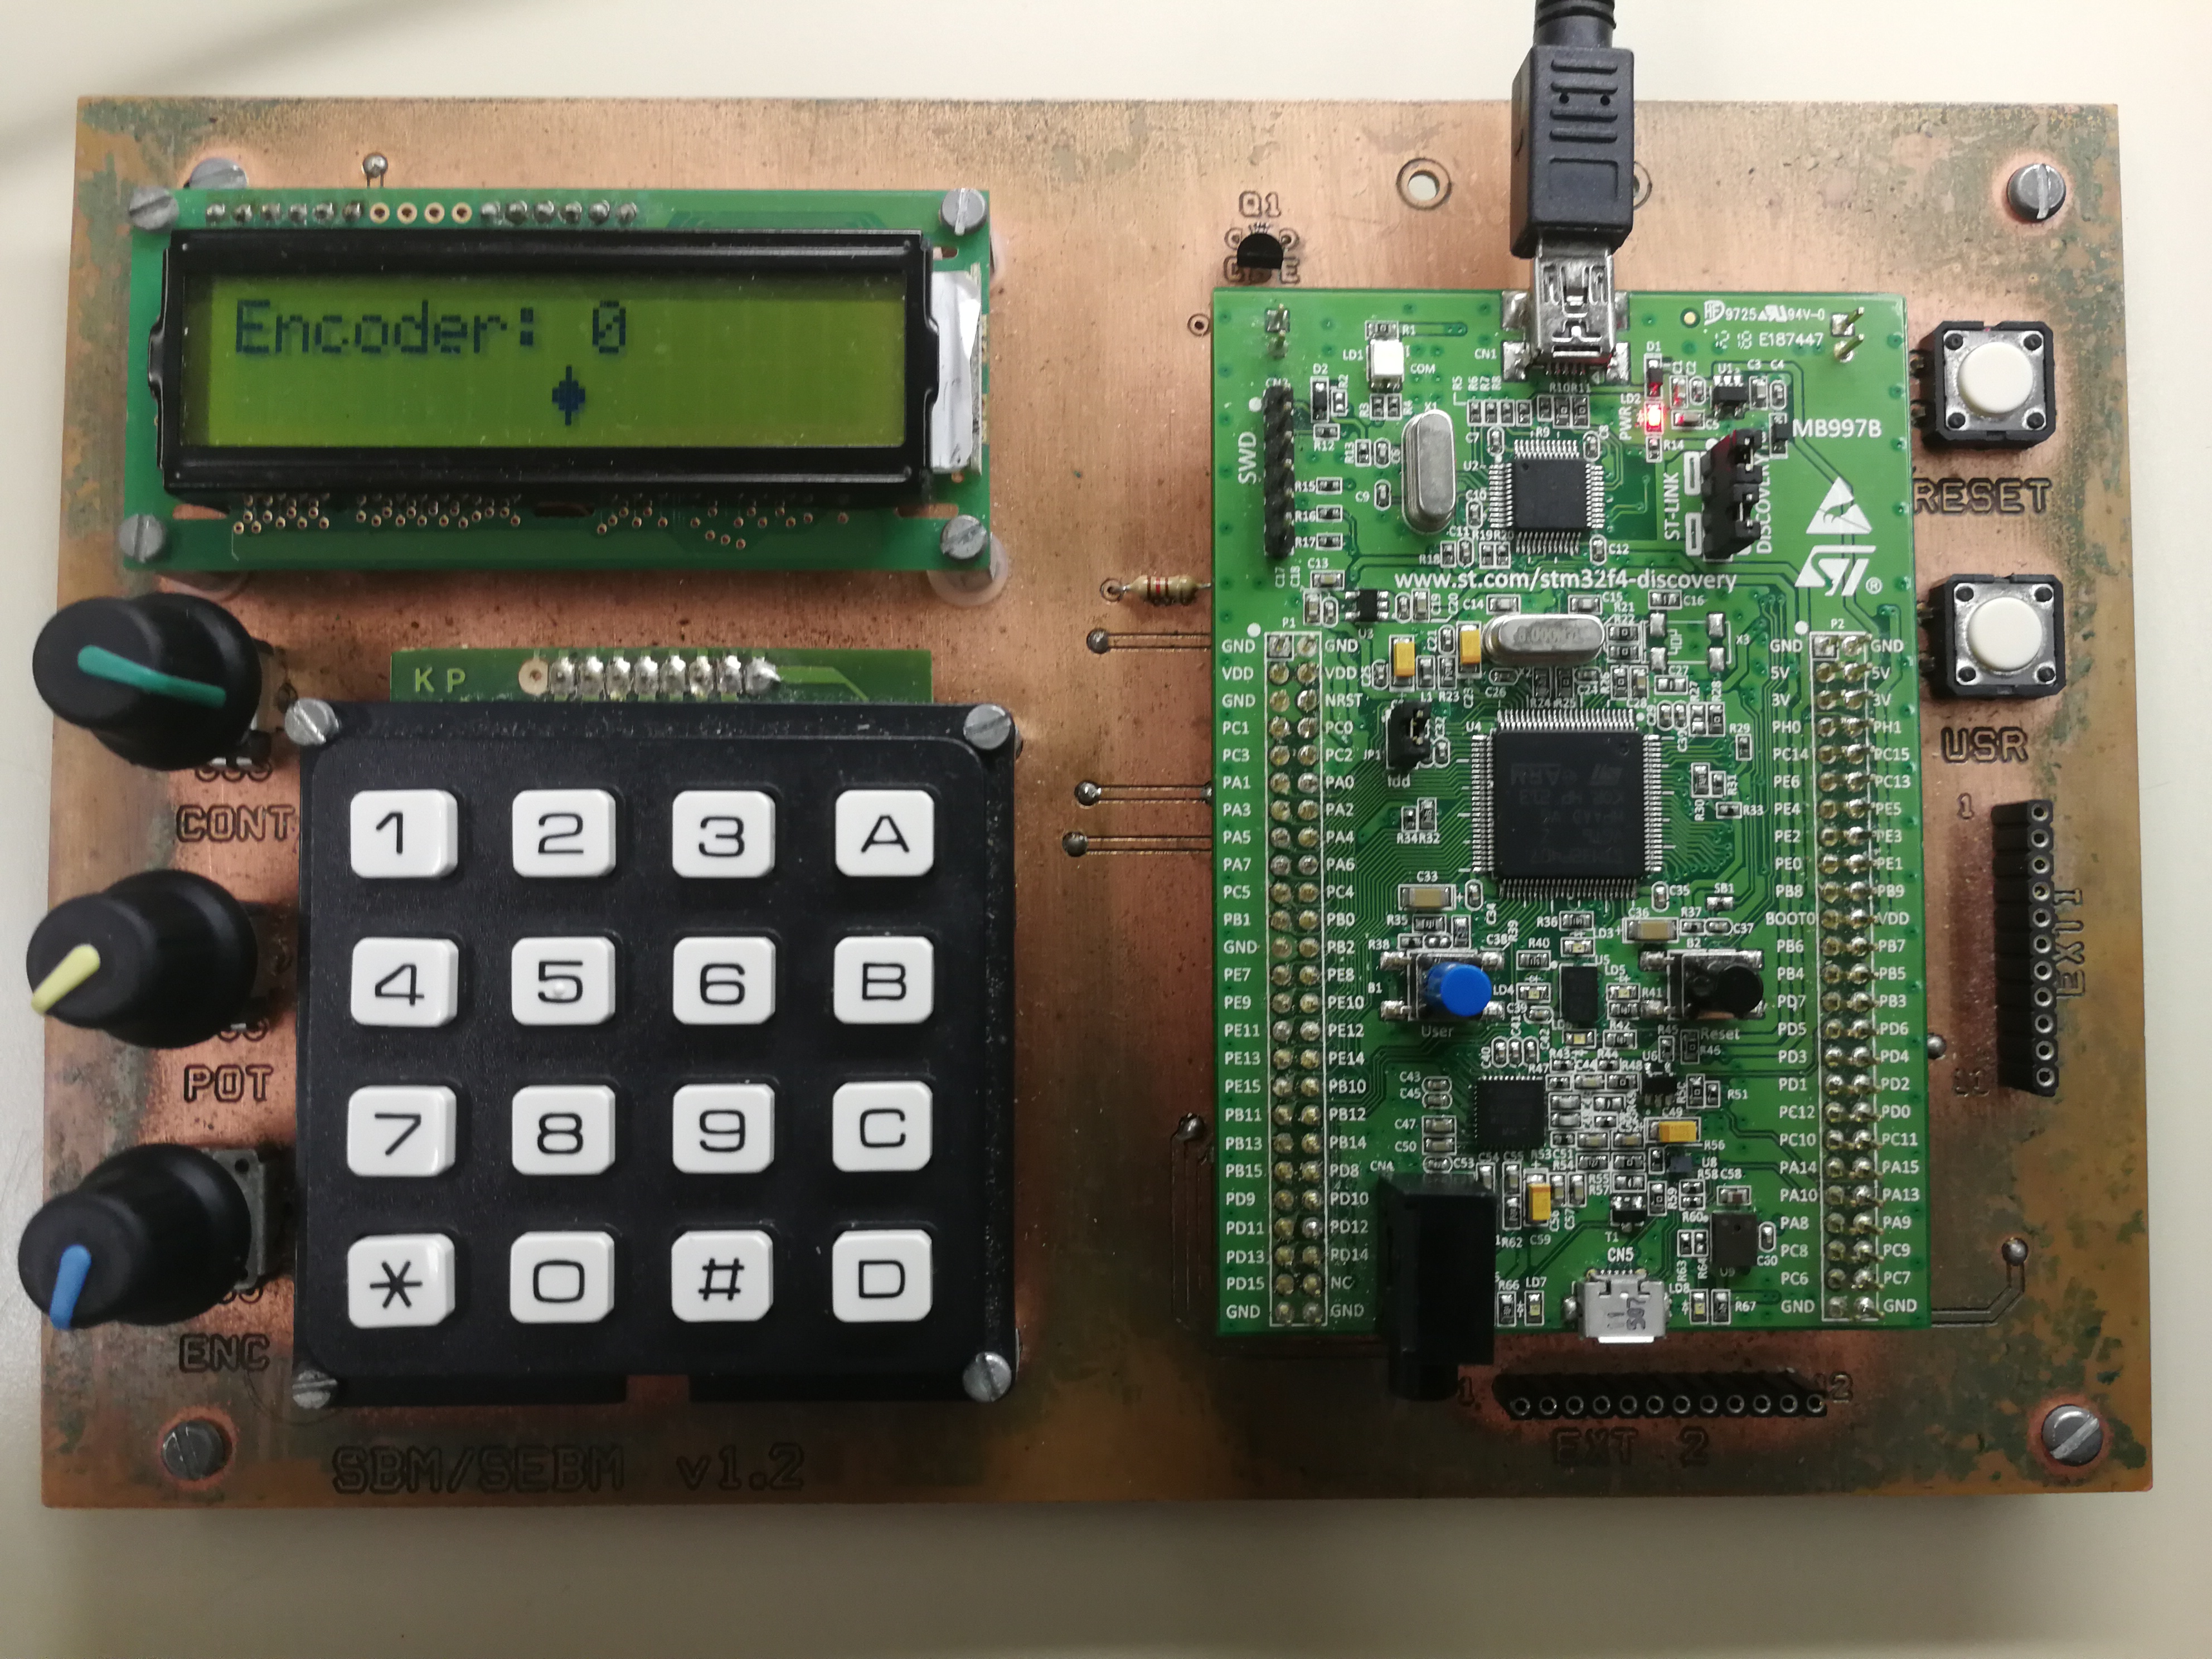
\includegraphics[width=.82\columnwidth]{../photos/board/c3-initial}
  \caption{ \label{fig:c3-board-initial} La placa mostrant el valor de l'encoder, en l'estat inicial. }
\end{figure}
\begin{figure}[p]
  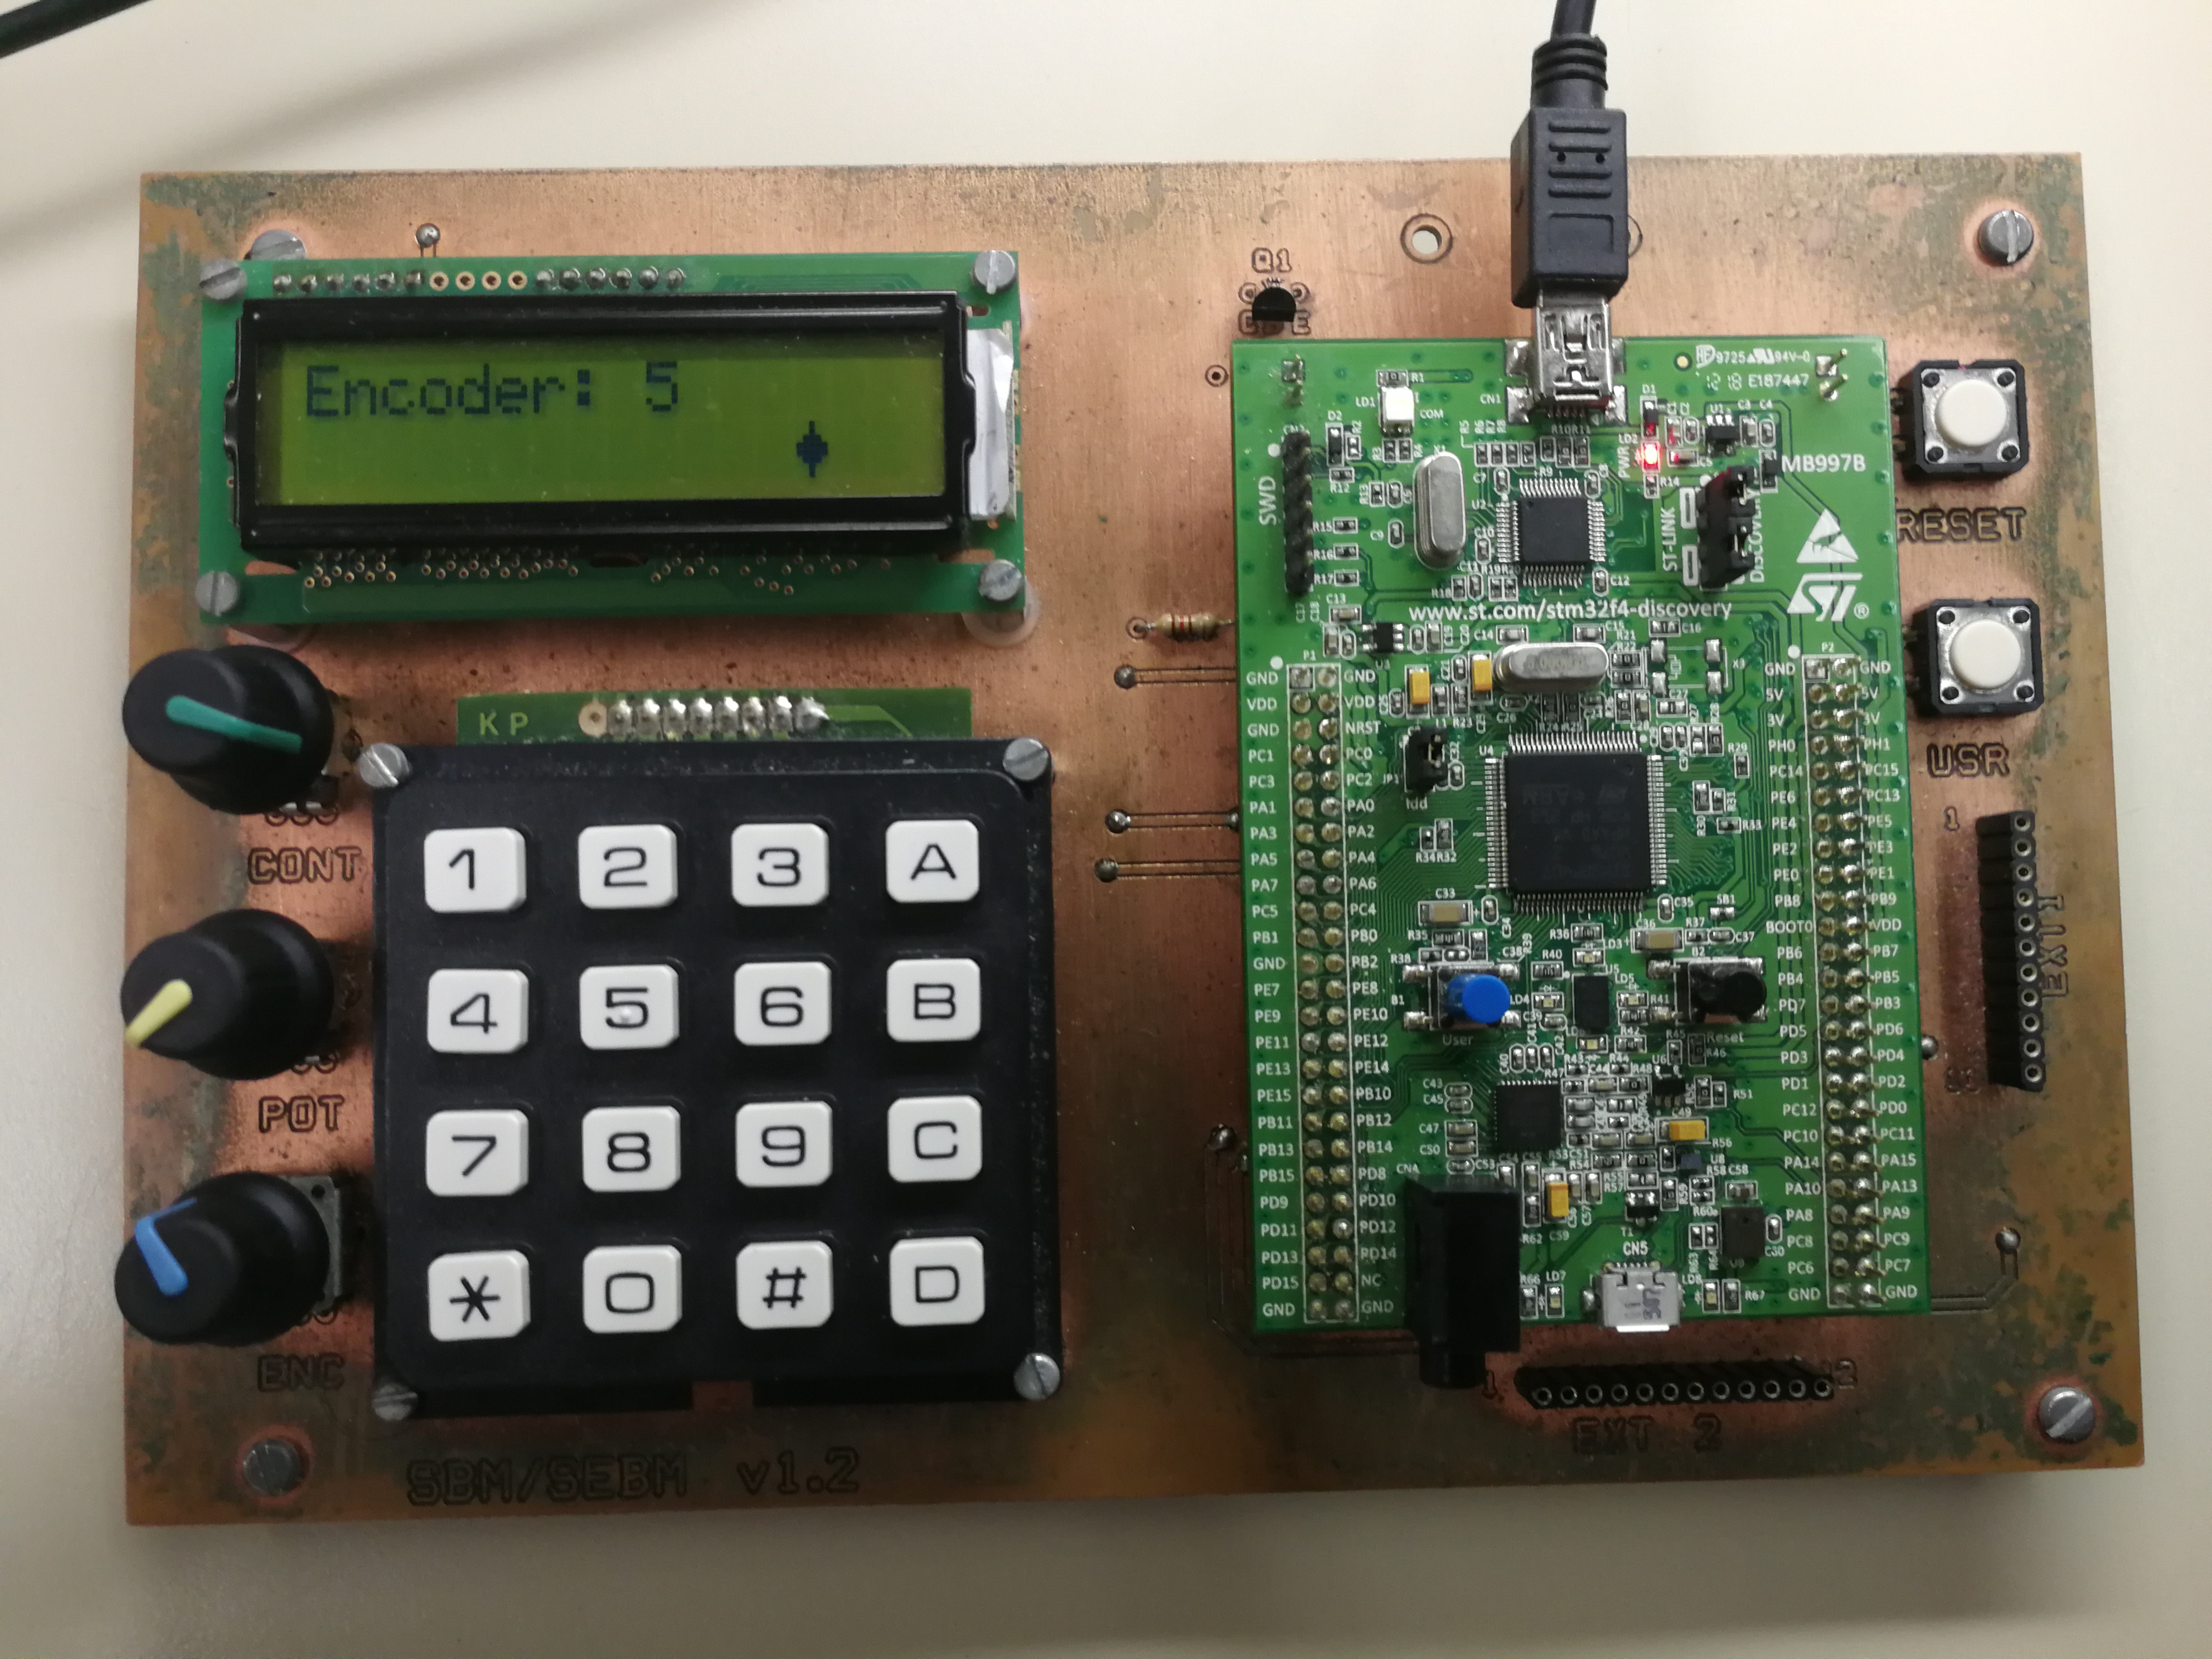
\includegraphics[width=.82\columnwidth]{../photos/board/c3-positive}
  \caption{ \label{fig:c3-board-positive} La placa mostrant un valor positiu de l'encoder. }
\end{figure}

\begin{figure}[p] %FIXME: subfigures?
  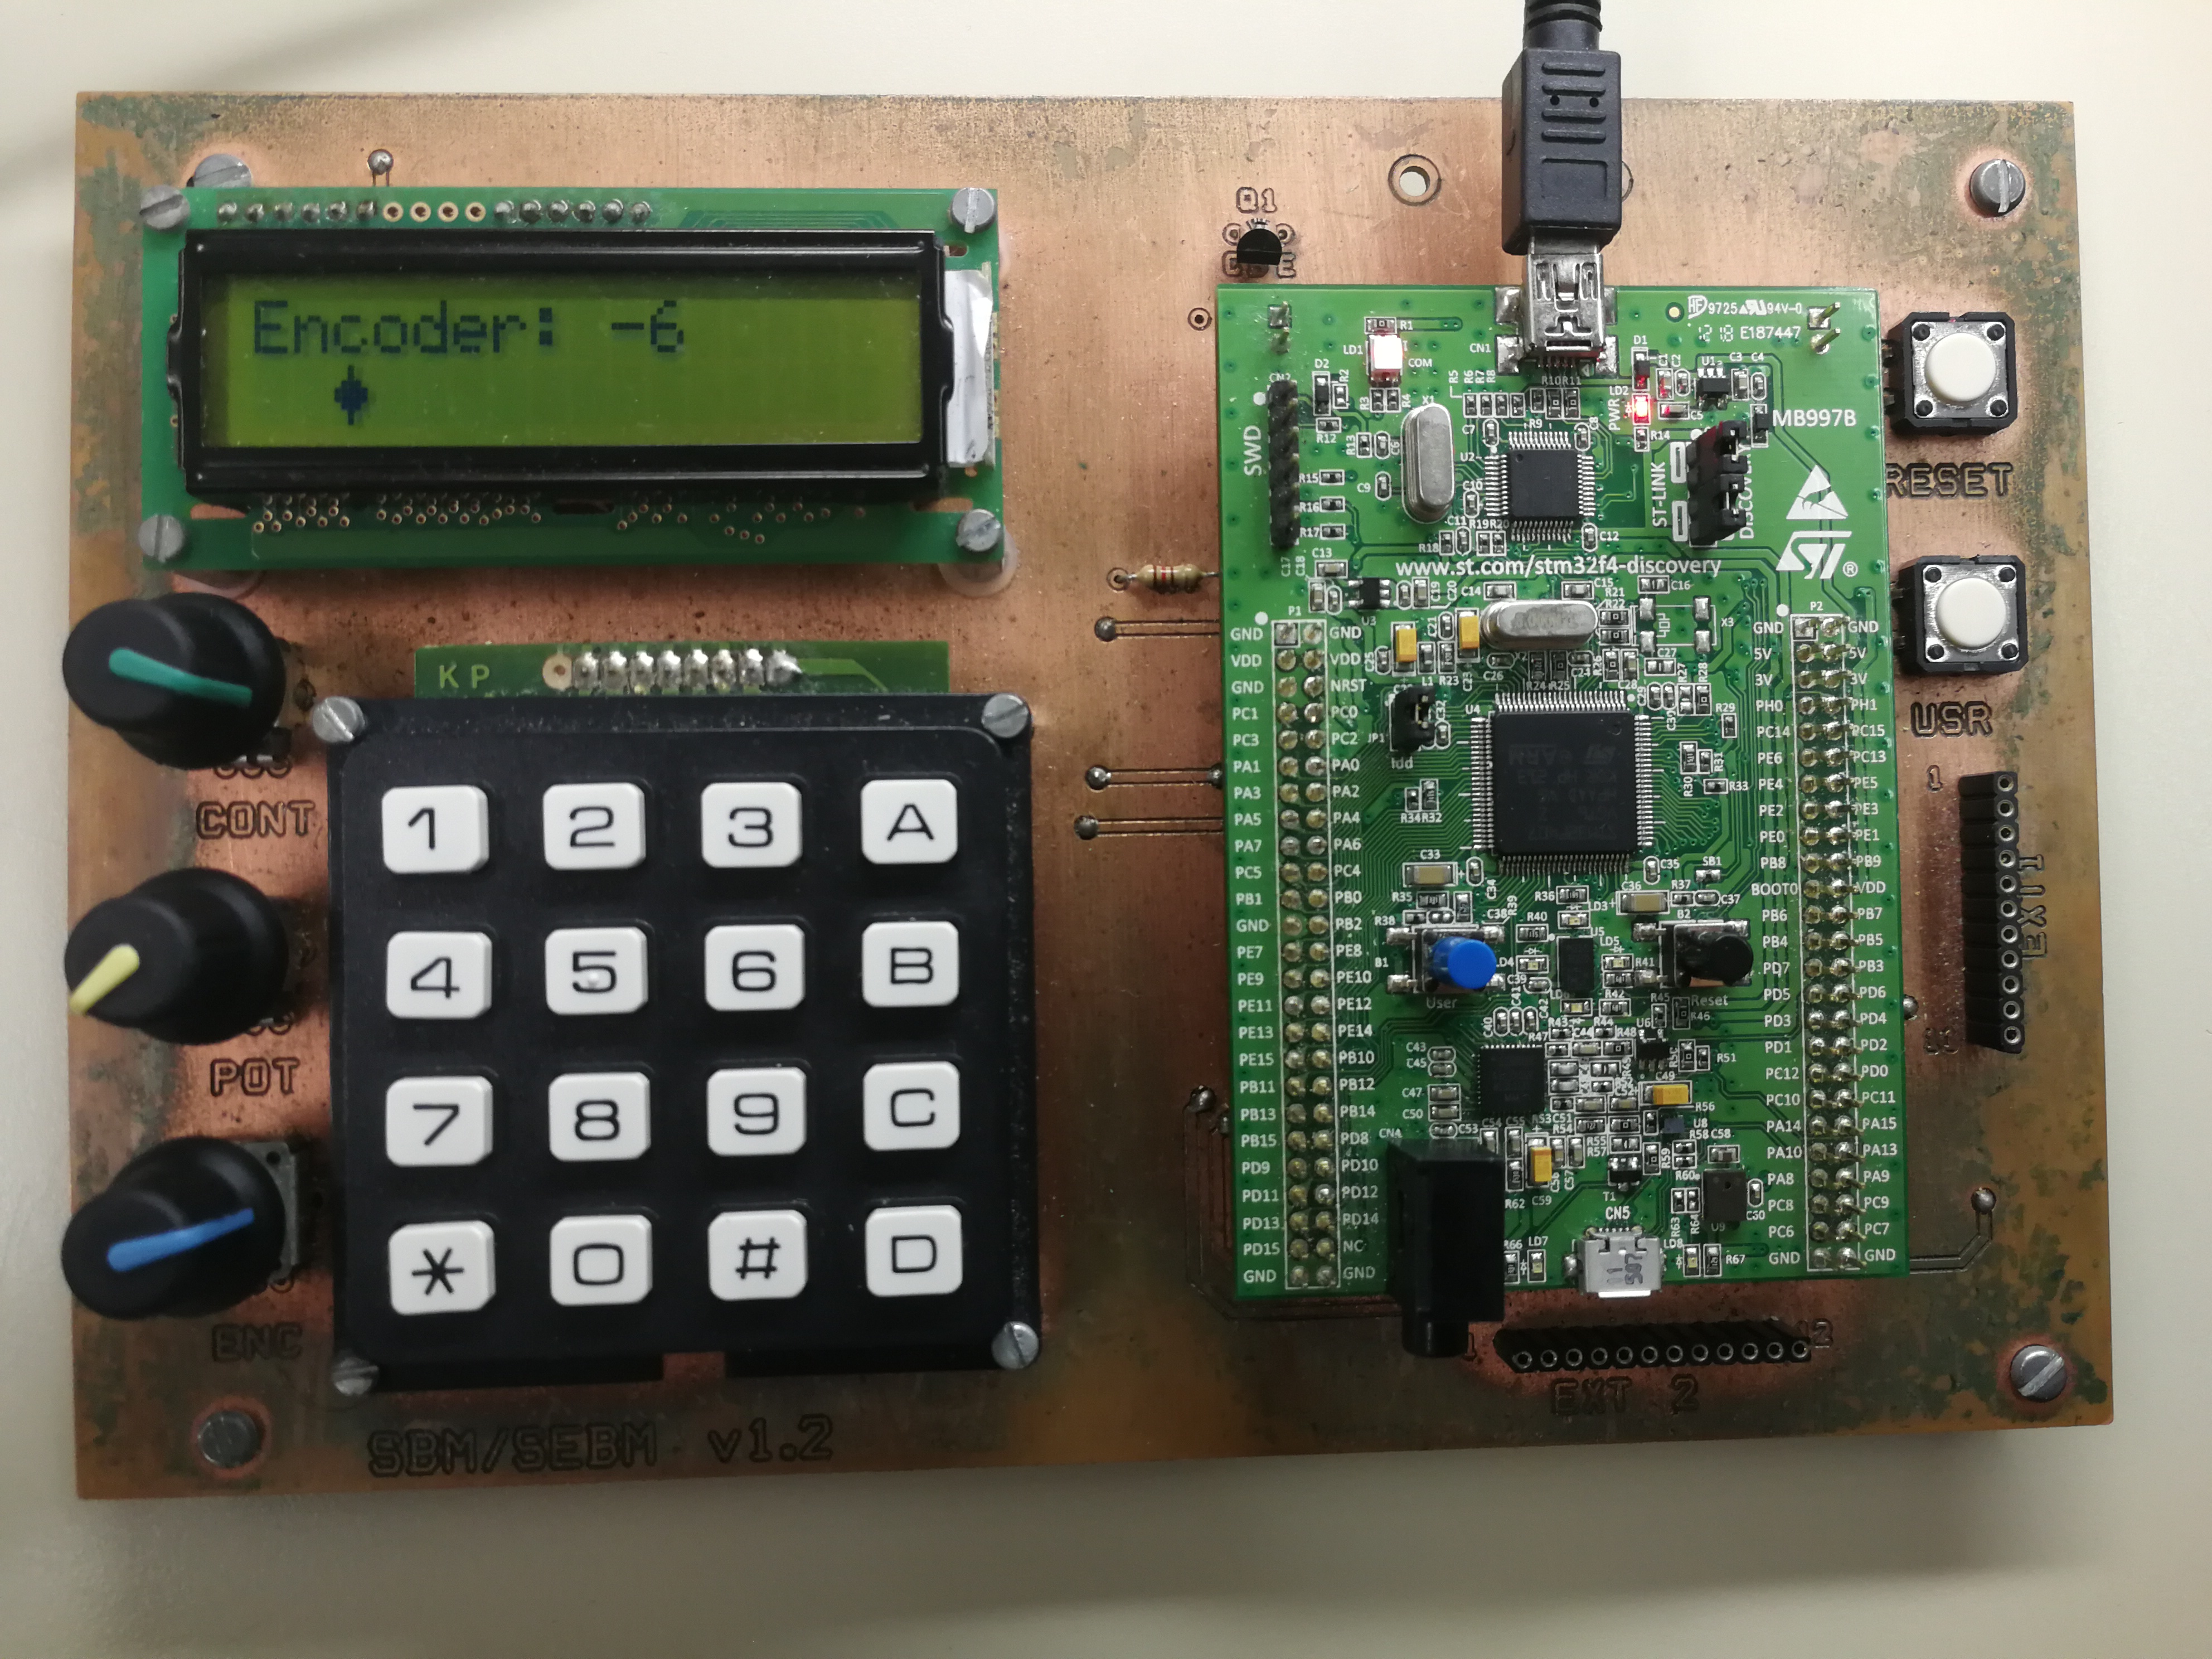
\includegraphics[width=.82\columnwidth]{../photos/board/c3-negative}
  \caption{ \label{fig:c3-board-negative} La placa mostrant un valor negatiu de l'encoder. }
\end{figure}
\begin{figure}[p]
  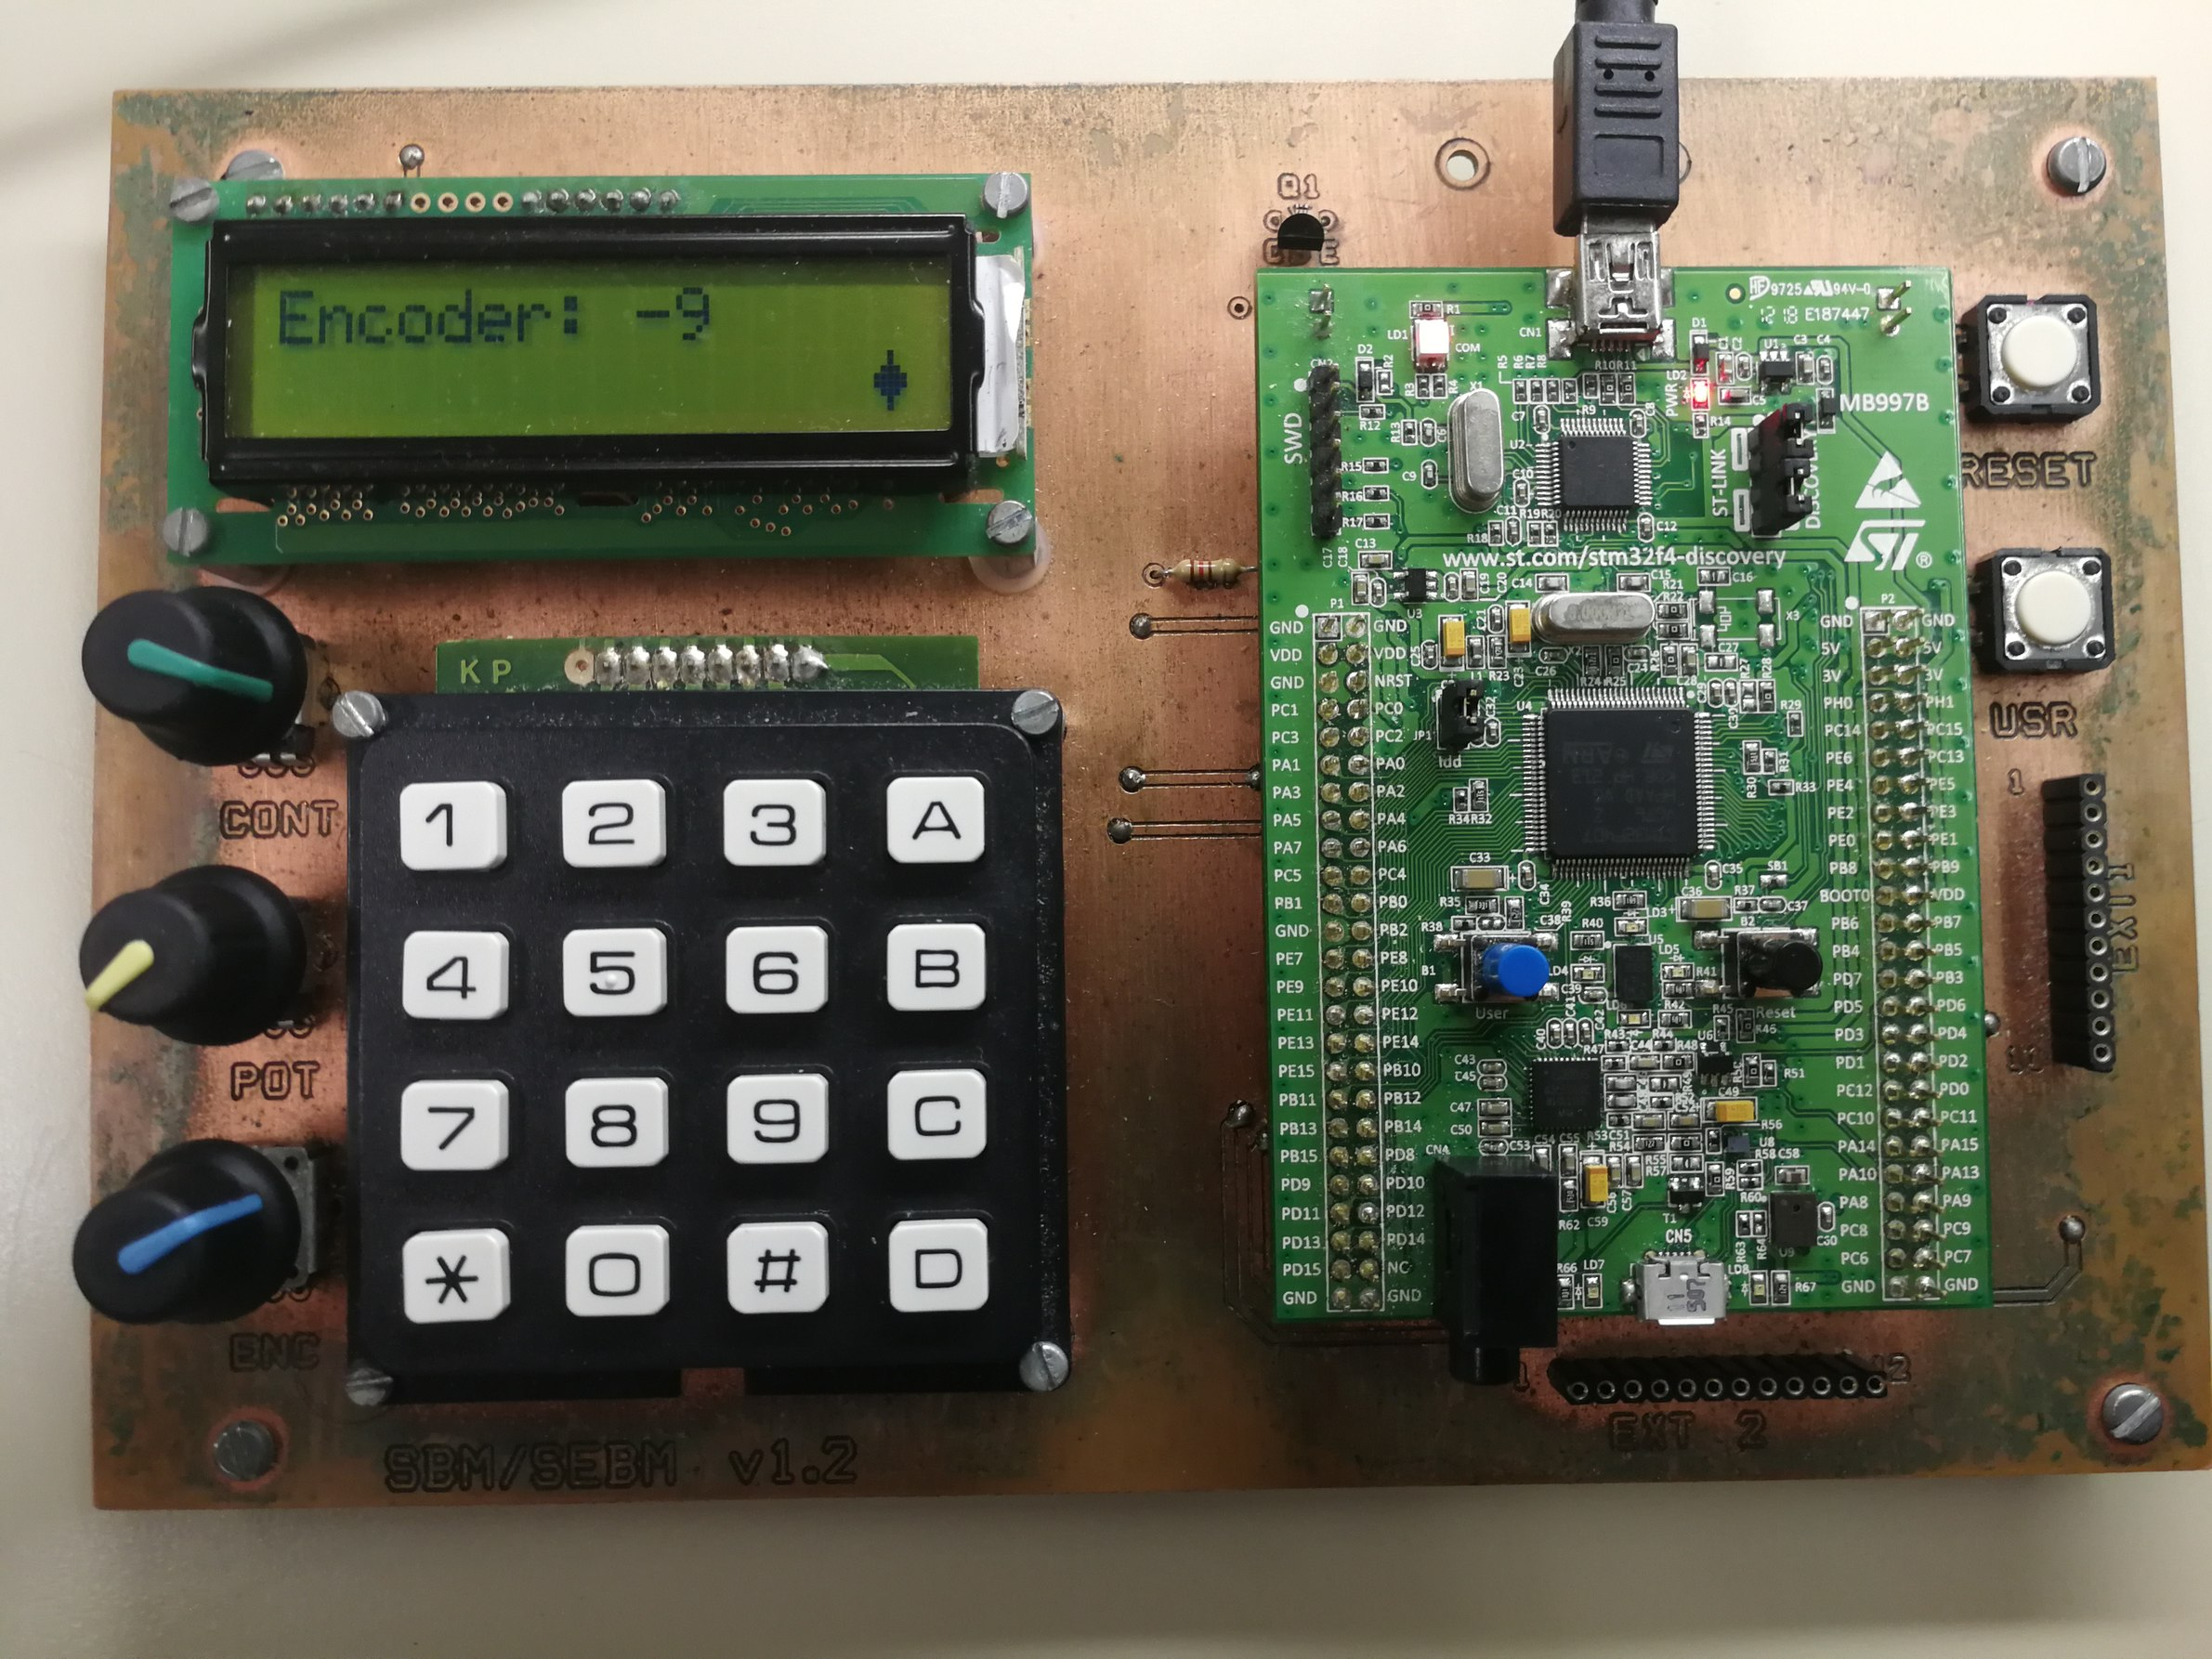
\includegraphics[width=.82\columnwidth]{../photos/board/c3-more-negative}
  \caption{ \label{fig:c3-board-more-negative} La placa mostrant un valor encara més negatiu de l'encoder. }
\end{figure}

Això conforma el \commit{34606834c5edd1805103dc5398f423e620f53be0}.


\section{Conclusió}

La pràctica s'ha realitzat sense problemes.

\section{Ajustaments posteriors}

Cap canvi a destacar.

